%% Outline
% 1. Navigation is important problem
% 1.5 Traditionally addressed by mapping during exploration and path
%      planning during exploitation.
% 2. End to end learning algorithms have shown promise to take over
%      mapping and path
% 3. We do not know how these algorithms work. There has been work in computer vision that shows the learning on neural network based methods can be learning totally different kind of patterns from what we would expect.
% 4.1 We find that it is not remembering the map it is being trained on
% 4.2 We find that no path planning is  happening only, memorizing and regeneration of the sequence of steps. However, it is not 

% 1. Navigation is important problem
% 1.5 Traditionally addressed by mapping during exploration and path
%      planning during exploitation.
Navigation remains a fundamental problems in mobile robotics and artificial intelligence~\cite{SmChIJRR1986,ElCOMPUTER1980}.
The problem is classically addressed by separating the eventual task of navigation into exploration, where the environment is represented in some sort of \emph{map} data-structure, and exploitation, where the map is used for localization and path-planning to find an optimal path to a given destination based on a given optimality criterion.  Although there have been many advances in this classical approach \cite{XXX}, it remains a difficult challenge: for example, mapping errors propagate to localization and path-planning tasks; monocular navigation remains a challenge in textureless or repeated texture environments 

More recently, end-to-end navigation methods---methods that attempt to  
solve the navigation problem without breaking it down into separate parts of localization, mapping and path-planning---have gained traction.
%
% 2. End to end learning algorithms have shown promise to take over
%      mapping and path-planning
With the recent success of Deep Reinforcement Learning (DRL) \cite{MnKaSiNATURE2015,MnKaSiNATURE2015}, these end-to-end navigation methods \cite{MnBaMiICML2016,SiHuMaNATURE2016,LePaKrISER2017,MiPaViICLR2017,OhChSiICML2016} forego decisions about the details that are required in the intermediate step of map building.  The potential for simpler yet capable methods is rich; for example, one can optimize to store only the minimal amount of map information that is required to optimally perform the end task of navigation.  One method \hl{XXX Give a citation from the list about (nominally, the method you will focus on in this paper) and a sentence about its great contribution or new capability.}
\begin{figure}[t!]%
\centering%
\def\figw{0.16\columnwidth}%
\newcommand{\includesnapshot}[1]{%
  \includegraphics[width=\figw,trim=336pt 0 0 0,clip]{#1}}%
\includesnapshot{images/snapshot/00063000-snapshot.png}%
\includesnapshot{images/snapshot/00087000-snapshot.png}%
\includesnapshot{images/snapshot/00156165-snapshot.png}%
\includesnapshot{images/snapshot/00159840-snapshot.png}%
\includesnapshot{images/snapshot/00166605-snapshot.png}%
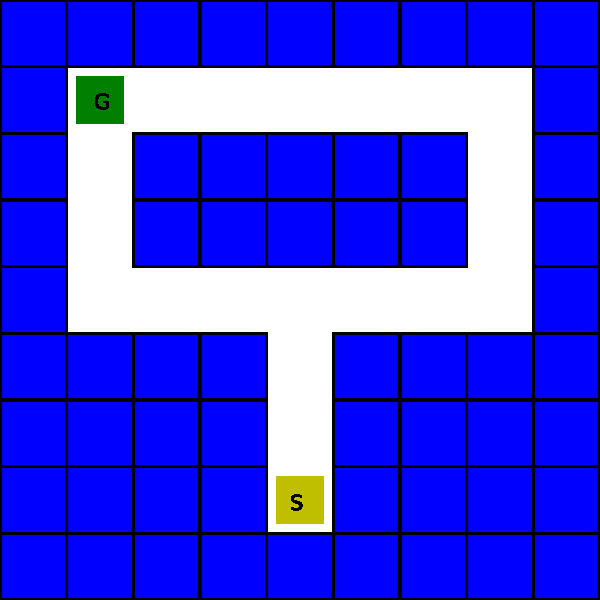
\includegraphics[width=\figw]{images/dhiman_0002_entityLayer.pdf}\\
\includesnapshot{images/snapshot/00193065-snapshot.png}%
\includesnapshot{images/snapshot/00338220-snapshot.png}%
\includesnapshot{images/snapshot/00344985-snapshot.png}%
\includesnapshot{images/snapshot/00948930-snapshot.png}%
\includesnapshot{images/snapshot/00956325-snapshot.png}%
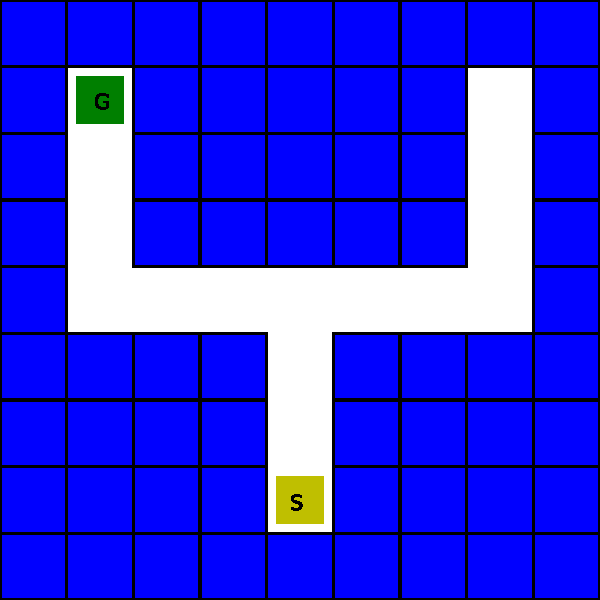
\includegraphics[width=\figw]{images/dhiman_0003_entityLayer.pdf}\\
\caption{A mazes sampled from the randomly generated mazes}%
\label{fig:environments}
\end{figure}


\hl{What role does Fig 1 play?  Figure this out and refer to it in the text}

% 3. We do not know how these algorithms work. There has been work in computer vision that shows the learning on neural network based methods can be learning totally different kind of patterns from what we would expect.
Despite this potential and recent successes, 
state-of-the-art DRL based methods have been confronted with their own set of problems, such as difficulty to understand the method limitations or the kind of patterns the algorithm is understanding.  The black-box nature of these methods make them hard to study.
On similar lines, \cite{NgYoClCVPR2015} show that neural-network-based object detection methods can be easily fooled by introducing noise that is imperceptible to humans. Hence, it is important to analyze the DRL methods to understand if they are truly ``learning to navigate'' \cite{MiPaViICLR2017}.

% 4.1 We find that it is not remembering the map it is being trained on
% 4.2 We find that no path planning is  happening only, memorizing and regeneration of the sequence of steps. However, it is not 
We analyze the navigation algorithm proposed in recent work \cite{MiPaViICLR2017}, to analyze if the trained agent (1) is able to navigate in unseen environments (2) is able perform fastest path planning.
Even though separting training and testing sets is the obvious thing to do in machine learning, we are the first work to evaluate any DRL based navigation method on unseen maps.

\hl{XXX there needs to be a quite more detailed explanation of the study setup and experiments here.  The reader should ``know the paper'' from only reading the introduction. XXX}

Our experiments give a clear answer of ``No'' to the posed question in the paper.
We find no evidence of DRL agents being able to perform shortest path-planning even in simple mazes. We observe that the agent prefers to take a particular path just as an artifact of initialization. We hypothesize that the agents are learning a correspondence between local sequence of frames and actions.  These findings are the results \hl{XXX tens of thousands of trials XXX}. We provide thorough and clear summary data to substantiate these findings as well as individual maps and results to explain them carefully.  A secondary finding is that even if the agent is trained on a single maze it is able to navigate better than random in unseen mazes. Furthermore, training the agent on randomly generated maps makes it generalize better to unseen mazes. 

